\documentclass[12pt]{article}
\usepackage{preamble}
\graphicspath{{pics/hw1/}}
\begin{document}
% \maketitle
\lhead{Problem Set 0}

%%%%%%%%%%%%%%%%%%%%%%%%%%%%%%%%%%%%%%%%%%%%%%%
%                  Definitions                %
%%%%%%%%%%%%%%%%%%%%%%%%%%%%%%%%%%%%%%%%%%%%%%%
%\includegraphics[width=\mywidth\textwidth]{}

% \begin{figure}[h!]
% \centering
% \input{pics/PS2/p7b}
% \caption{}
% \label{fig-}
% \end{figure}

% \begin{enumerate}[label=\alph*.]
%     \setcounter{enumi}{1}
%     \item 
% \end{enumerate}
\renewcommand{\vem}{\newpage}

\newcommand\independent{\protect\mathpalette{\protect\independenT}{\perp}}
\def\independenT#1#2{\mathrel{\rlap{$#1#2$}\mkern2mu{#1#2}}}

%%%%%%%%%%%%%%%%%%%%%%%%%%%%%%%%%%%%%%%%%%%%%%%
%                Problem 1                    %
%%%%%%%%%%%%%%%%%%%%%%%%%%%%%%%%%%%%%%%%%%%%%%%
\problem{1. Randomized  Controlled  Trial -- It begins...}{
You  have  a  randomized  controlled  trial  (RCT)  with  potential  outcomes $Y_i(0)$, $Y_i(1)$ and  treatment $D_i$.   Let $P(D_i =  1)  =  0.5$  and  let $i = 1,...,N$.   You  observe 
$Y_i = Y_i(0) \cdot (1-D_i) + Y_i(1) \cdot D_i$.
    \begin{enumerate}[label=(\alph*)]
    \item Consider a regression of $Y_i$ on $D_i$.  Prove that the regression of $Y_i$ on $D_i$ estimates ATE. Does it estimate TOT too?  If so, prove that.
    \end{enumerate} 
}
\def\yi{Y_i(0)(1-D_i) + Y_i(1)D_i}

\begin{align*}
\intertext{Taking a hint from Joel, we have linear CEF given $D_i$ is binary meaning we have a saturated model.}
\E{Y_i \cond D_i} &= \alpha + \tau D_i
\intertext{Then the average treatment effect estimate $\tau$ from this regression is an unbiased estimator for}
\tau &= (\alpha+\tau) - \alpha \\
    &= \E{Y_i \cond D_i=1} - \E{Y_i \cond D_i=0} \\
    &= \E{\yi \cond D_i=1} - \E{\yi \cond D_i=0} \\
    &= \E{Y_i(1) \cond D_i=1} - \E{Y_i(0) \cond D_i=0}
\shortintertext{and because $D$ is randomly assigned, $Y_i(1),Y_i(0)\perp D_i$, so $\E{Y_i(0) \cond D_i=0}=\E{Y_i(0)}$ and $\E{Y_i(1) \cond D_i=1}=\E{Y_i(1)}$}
    &= \E{Y_i(1)} - \E{Y_i(0)} \\
    &= \overline\tau_{ATE}
\end{align*}


% \def\xi{
%     \begin{pmatrix}
%     1 & D_i
%     \end{pmatrix}
% }
% \def\xiprime{
%     \begin{pmatrix}
%     1 \\ D_i
%     \end{pmatrix}
% }
% \def\xiprimexi{
%     \begin{pmatrix}
%     D_i^2 & -D_i \\
%     -D_i & 1
%     \end{pmatrix}
% }
% \def\gamma{\frac{1}{P(1-P)}}
% \begin{align*}
% \intertext{The OLS estimator $\hat\beta$ converges to}
% \hat\beta \to &(\E{X_i' X_i})^{-1}\E{X_i' Y_i}
% \intertext{So regressing $Y_i$ on $D_i$ and a constant would yield the estimator}
% \hat\beta \to &\E{\xiprime\xi}^{-1}\E{\xiprime Y_i} \\
%     &= \frac{1}{\E{D_i} - \E{D_i}^2}\E{\xiprimexi}
%         \E{\begin{pmatrix} Y_i \\ D_i Y_i \end{pmatrix}}
% \intertext{Let $P\equiv P(D_i=1)$, then $\E{D_i^2}=\E{D_i}=P$ and }
%     &= \frac{1}{P(1-P)}
%         \E{\begin{pmatrix} P & -P \\ -P & 1 \end{pmatrix}}
%         \E{\begin{pmatrix} Y_i \\ D_i Y_i \end{pmatrix}}\\
%     &= \frac{1}{P(1-P)}
%         \E{\begin{pmatrix} P\E{Y_i} -P\E{D_i Y_i} \\ \E{D_i Y_i} - P\E{Y_i} \end{pmatrix}}
% \intertext{So the estimated treatment effect from this regression would converge to}
% \hat\beta_1 \to &\frac{1}{P(1-P)}\left[ \E{D_i Y_i} - P\E{Y_i}\right] \\
% \intertext{and}
%     \E{D_i Y_i} - P\E{Y_i} &= \E{Y_i (D_i - P)} \\
%     &= \E{\E{Y_i (D_i - P) \cond D_i}} \\
%     &= \P(D_i=0)\E{Y_i (D_i - P) \cond D_i=0} +  \P(D_i=1)\E{Y_i (D_i - P) \cond D_i=1} \\
%     &= (1-P)\E{Y_i(-P) \cond D_i=0} +  P\E{Y_i(1-P) \cond D_i=1} \\
%     &= (1-P)(-P)\E{Y_i \cond D_i=0} +  P(1-P)\E{Y_i \cond D_i=1} \\
%     &= P(1-P)\left\{ \E{Y_i \cond D_i=1} - \E{Y_i \cond D_i=0} \right\}\\
%     &= P(1-P)\left\{ \E{Y_i(1) \cond D_i=1} - \E{Y_i(0) \cond D_i=0} \right\}\\
% \intertext{Because $D_i$ is randomly assigned, it is independent of the potential outcomes, and we can assume that
% $\E{Y_i(1) \cond D_i=1} = \E{Y_i(1)}$ and $\E{Y_i(0) \cond D_i=0} = \E{Y_i(0)}$, so}
%     &= P(1-P)\left\{ \E{Y_i(1)} - \E{Y_i(0)} \right\}\\
% \intertext{So the regression coefficient converges to (and is an unbiased estimator for)}
% \hat\beta_1 \to &  \gamma P(1-P)\left\{ \E{Y_i(1)} - \E{Y_i(0)} \right\}\\
%     &= \E{Y_i(1)} - \E{Y_i(0)}
% \intertext{Thus the regression of $Y_i$ on $D_i$ and a constant estimates the ATE.}

\begin{align*}
\intertext{Additionally, because treatment assignment is random, the average treatment effect becomes}
\overline{\tau}_{ATE} &= \E{Y_i(1)} - \E{Y_i(0)} \\
    &= \E{Y_i(1) \cond D_i=1} - \E{Y_i(0) \cond D_i=1} \\
    &= \overline{\tau}_{TOT}
\intertext{and is also estimated by the regression.}
\end{align*}


%%%%%%%%%%%%%%%%%
%     Part b    %
%%%%%%%%%%%%%%%%%
\vem
\problem{}{
    \begin{enumerate}[label=(\alph*)]
    \setcounter{enumi}{1}
    \item Does setting $P(D_i= 1) = 0.5$ maximize the power (i.e.  minimize the standard error of the estimated treatment effect) in your RCT? Prove.  (You may take the formula for $Var(\hat{\beta}_{OLS})$ as given; feel free to look it up if you do not recall it.)
    \end{enumerate} 
}
\def\D{\mathbf{D}}
\def\X{\begin{pmatrix} 1_{n\times 1} & \D \end{pmatrix}}
\def\Xprime{\begin{pmatrix} 1_{1\times n} \\ \D' \end{pmatrix}}
\def\XprimeX{
    \begin{pmatrix}
    n & \sum_{i=0}^n D_i \\ \sum_{i=0}^n D_i & \sum_{i=0}^n D_i^2
    \end{pmatrix}}
\def\XprimeXinv{
    \frac{1}{n\sum_{i=0}^n D_i^2 - \left( \sum_{i=0}^n D_i \right)^2}
    \begin{pmatrix}
    \sum_{i=0}^n D_i^2 & -\sum_{i=0}^n D_i \\ -\sum_{i=0}^n D_i & n
    \end{pmatrix}}

\begin{align*}
    \intertext{Given a simple univariate OLS, and given D is distributed with binomial, whose variance can be asmptotically approximated by $np(1-p)$,}
    Var(\hat{\beta_{OLS}}) &= \frac{\sigma_u^2}{SST_D} \\
                           &= \frac{\sigma_u^2}{np(1-p)} \\
    \intertext{Minimizing the above expression w.r.t. p is equivalent to maximizing $p(1-p)$ w.r.t. p. Hence, $p^* = 0.5$}
\end{align*}

%\begin{align*}
%\intertext{From Greene (2012, pp. 61), if $\sigma^2$ is the variance of the residuals, then we know the exact variance of the OLS estimator is}
%Var[\hat\beta_{OLS}] &= \sigma^2 \E{(X' X)^{-1}} \\
%    &= \sigma^2 \E{\left(\Xprime \X \right)^{-1}} \\
%    &= \sigma^2 \E{\XprimeX ^{-1}}\\
%    &= \sigma^2 \E{\XprimeXinv}
%\shortintertext{where $1_{1\times n}$ is a column vector of ones and $\D$ is the treatment assignment column vector. %Then the variance of the treatment estimator $\hat\beta_1$ is the bottom-right element of the variance matrix:}
%Var[\hat\beta_1 ] 
%    &= \sigma^2 \E{\frac{n}{n\sum_{i=0}^n D_i^2 - \left( \sum_{i=0}^n D_i \right)^2}} \\
%    &= \sigma^2 \E{\frac{1}{\sum_{i=0}^n D_i^2 - \frac{1}{n} \left( \sum_{i=0}^n D_i \right)^2}} \\
%\end{align*}




%%%%%%%%%%%%%%%%%
%     Part c    %
%%%%%%%%%%%%%%%%%
\vem
\problem{}{
    \begin{enumerate}[label=(\alph*)*]
    \setcounter{enumi}{2}
        \item Suppose you also observe covariates $X_i$.  You are concerned about heteroskedaticity and estimate a regression of  $\hat{\varepsilon}^2_i$ on $X_i$, where  $\hat{\varepsilon_i}$ are OLS residuals from regressing $Y_i$ on $X_i$.  Using the fitted values from this regression you form weights $w_i= 1/\hat{\sigma_i}$ and reweight your data.  Prove that a regression of $Y^w_i$ on $D^w_i$, where a $w$ superscript signifies a reweighted variable, does not necessarily estimate ATE. Does it estimate TOT?
    \end{enumerate} 
}



%%%%%%%%%%%%%%%%%
%     Part d    %
%%%%%%%%%%%%%%%%%
\vem
\problem{}{
    \begin{enumerate}[label=(\alph*)]
    \setcounter{enumi}{3}
        \item Assuming your model of heteroskedasticity is correct,  name one advantage and one disadvantage of the weighted regression (versus OLS). You may rely on results you’ve learned from previous econometrics courses.
    \end{enumerate} 
}

Advantage: In ARE 212, we learned that under heteroskedasticity, OLS is no longer the minimum variance estimator among the class of linear and unbiased estimators. Weighting solves above issue and reduces standard errors on the coefficients.

Disadvantage: Weighted least squares requires one to know exactly what the weights should be (given the interpretation you're looking for). Otherwise, picking the wrong weights (for the question) will risk skewing the results in unwanted ways. For instance, even if you have correctly modeled the heteroskedasticity, if you have an outlier observation that shares regressor values that are similar to other observations with low error, then WLS would give this outlier too much weight. In an attempt to approach the right weights, one can use iterative WLS.
Using WLS may also lead to a misinterpretation of the treatment effect since outlier treated observations will be given less weight when we may care most about them. All depends on our intended interpretation!


%%%%%%%%%%%%%%%%%
%     Part e    %
%%%%%%%%%%%%%%%%%
\vem
\problem{}{
    \begin{enumerate}[label=(\alph*)]
    \setcounter{enumi}{4}
        \item Suppose that it costs \$1 to generate each control observation and \$4 to generate each treated observation (i.e.  the treatment itself is expensive).  You have a total budget of \$150.  To maximize power in your RCT, how many observations will you assign to treatment, and how many will you assign to control?  (To be clear, your  estimator  here  will  be  an  OLS regression of $Y_i$ on $D_i$,  not  the  re-weighted regression.)
    \end{enumerate} 
}


\begin{align*}
\intertext{Utilizing equation in part(b), we want to maximize $np(1-p)$, where $p$ is probability of treatment.}
\intertext{Define budget constraint:}
    150 &= 4np + n(1-p) \\
        &= n (3p+1)
\intertext{Given above budget constraint, we can write the following maximization problem:}
    & \max_{p,n} np(1-p) \;\; \text{s.t.} \;\; n (3p+1) = 150 \\
    &\iff \max_{p} \frac{150}{3p+1} p(1-p) \\
    &\iff \max_{p} \frac{150}{3p+1} (p-p^2)
\intertext{Solving the FOC w.r.t. p, we achieve the following:}
    p &= + \frac{1}{3} \;\; \text{or} \;\; -1
\intertext{p clearly cannot be negative. Hence, $p^* = \frac{1}{3}$, $N^* = 75$, $N^*(Trt) = 25$, and $N^*(Cont) = 50$}
\end{align*}


\newpage
%%%%%%%%%%%%%%%%%%%%%%%%%%%%%%%%%%%%%%%%%%%%%%%
%                Problem II                   %
%%%%%%%%%%%%%%%%%%%%%%%%%%%%%%%%%%%%%%%%%%%%%%%
\problem{2. Randomized  Controlled  Trial -- Here we go again!}{
We continue to use the RCT discussed above, but you no longer have any covariates $X_i$ (and you can forget about the weights and costs).  You may assume $P(D_i= 1) = 0.5$. Suppose $Y_i$ is missing for some observations (but $D_i$ is complete for all observations).  might happen because, for example, some participants in the RCT did not respond to the survey collecting the outcome data.
\vem
    \begin{enumerate}[label=(\alph*)]
        \item First assume $Y_i$ are missing at random.  Propose a simple test for this hypothesis. Does a regression of $Y_i$ on $D_i$ (using complete observations) estimate ATE if your assumption is correct?
    \end{enumerate} 
}

\begin{align*}
\intertext{Let $M_i$ be an indicator for  of $Y_i$, i.e., $M_i=1$ if $Y_i$ is missing and $M_i=0$ if $Y_i$ is not missing. In this setting, missing at random would mean that the missing data process is independent of $Y_i$ and $D_i$. Because we have no other data to compare the distribution of $Y_i$ to, we cannot test if the missing data process is independent of $Y_i$. However, by running a regression of $M_i$ on $D_i$, we can test for linear correlation between missingness and treatment assignment. So a simple test could include running the following regression}
M_i = \beta_0 + \beta_1 D_i +\epsilon_i
\intertext{and checking if $\beta_1$ is significantly different from zero. If $\beta_1$ is significantly different from zero, we have evidence that the Missing At Random assumption is violated.}
\intertext{Under the Missing At Random assumption, the regression of $Y_i$ on $D_i$ still estimates ATE.}
\end{align*}




%%%%%%%%%%%%%%%%%
%     Part b   %
%%%%%%%%%%%%%%%%%
\vem
\problem{}{
    \begin{enumerate}[label=(\alph*)]
    \setcounter{enumi}{1}
        \item If the $Y_i$ are missing at random,  does your test have the correct size?  That is, does it reject at a rate $\alpha= 0.05$?  Briefly explain.
    \end{enumerate} 
}

If the data are missing at random, the test of Missing at Random has the correct size because the regression would only include the complete observations. 




%%%%%%%%%%%%%%%%%
%     Part c   %
%%%%%%%%%%%%%%%%%
\vem
\problem{}{
    \begin{enumerate}[label=(\alph*)]
    \setcounter{enumi}{2}
        \item If the null hypothesis is false (i.e. the $Y_i$ are not missing at random), will your test necessarily reject as $N \to \infty$?
    \end{enumerate} 
}

One of the ways that the missingness could not be random is if the missing data process is related to the value of $Y_i$. Because we only observe the $Y_i$ we collect, and the simple test above only tests for a relationship between missingness and the treatment, any missingness related to $Y_i$ would not be detected and the test will not necessarily reject at $N\to\infty$.


\newpage
%%%%%%%%%%%%%%%%%%%%%%%%%%%%%%%%%%%%%%%%%%%%%%%
%                Problem 3                    %
%%%%%%%%%%%%%%%%%%%%%%%%%%%%%%%%%%%%%%%%%%%%%%%
\problem{3. The Roy Model (Selection)}{
We now consider a gentle introduction to the selection model known as the Roy Model.  discussed this model briefly in class in the context of choosing fishing versus hunting. The key assumption in the Roy Model is that individuals select into treatment based on their gains (or expected gains) from treatment. This assumption comes naturally from a framework in which individuals maximize utility, but, to be clear, it is an assumption (i.e.  there is no guarantee it holds in your real-world data). To fix ideas, assume a binary treatment $D_i$ and potential outcomes $Y_i(0)$ and $Y_i(1)$. Let the treatment gain for individual $i$ be equal to $i$’s treatment effect, $\tau_i=Y_i(1)-Y_i(0)$. Assume $i$ selects into treatment if and only if $\tau_i>0$ (i.e. $D_I=\textbf{1}(\tau_i>0))$. \\

For part $(d)$ of this question you may take as known a result we refer to as the inverse Mills ratio — if $A \sim N(0,1)$, then $E[A \cond A > c] = \frac{\phi(c)}{1-\Phi(c)}$ (we will show this in lecture). \\

    \begin{enumerate}[label=(\alph*)]
    \item First assume $Y_i(0) =c$.  Show that a regression of $Y_i$ on $D_i$ estimates TOT.
    \end{enumerate} 
}

\begin{align*}
\intertext{The regression of $Y_i$ on $D_i$ is}
\E{Y_i|D_i} = \alpha + \tau D_i
\intertext{So the treatment effect estimated by the regression is}
\tau &= (\alpha+\tau) - \alpha \\
    &= \E{Y_i \cond D_i=1} - \E{Y_i \cond D_i=0} \\
    &= \E{Y_i(1) \cond D_i=1} - \E{Y_i(0) \cond D_i=0} \\
    &= \E{Y_i(1) \cond D_i=1} - \E{c \cond D_i=0} \\
    &= \E{Y_i(1) \cond D_i=1} - \E{c \cond D_i=1} \\
    &= \E{Y_i(1) \cond D_i=1} - \E{Y_i(0) \cond D_i=1} \\
    &= \overline{\tau}_{TOT}
\end{align*}


%%%%%%%%%%%%%%%%%
%     Part b    %
%%%%%%%%%%%%%%%%%
\vem
\problem{}{
    \begin{enumerate}[label=(\alph*)*]
    \setcounter{enumi}{1}
    \item Now let $Y_i(0)$ and $Y_i(1)$ be independent with marginal Uniform(0,1) distributions. Analytically derive $E[Y(1)_i \cond D_i= 1]$ and $E[Y(0)_i \cond D_i= 0]$. Does a regression of $Y_i$ on $D_i$ estimate TOT?
    \end{enumerate} 
}

%Given $Y_i(0) ~ U[0,1]$ , $Y_i(1) ~ U[0,1]$, and $Y_i(0) \independent Y_i(1)$
%\begin{align*}
%P[Y_i(1) < y | Y_i(0) < Y_i(1)] &= \frac{P[Y_i(0) < Y_i(1) < y]}{P[Y_i(0) < Y_i(1)]} \\
%                                &= \frac{\int_{0}^{y} [\int_{0}^{y} f(Y_i(0),Y_i(1)) \: dY_i(1)] \; dY_i(0)}{0.5} \\
%                                &= \frac{\int_{0}^{y} [\int_{0}^{y} 1 \: dY_i(1)] \; dY_i(0)}{0.5} \\ 
%                                &= \frac{\int_{0}^{y} y \; dY_i(0)}{0.5} \\
%                                &= \frac{0.5 y^2}{0.5} \\
%                                &= y^2 \\
%\intertext{}
%P[Y_i(1) = y | Y_i(0) < Y_i(1)] &= 2y
%\intertext{}
%\E{Y_i(1)|D_i=1} &= E[Y_i(1) | Y_i(0) < Y_i(1)] \\
%                 &= \int_{0}^{1} y \: P(Y_i(1) | Y_i(0) < Y_i(1)) \: dy \\
%                 &= \int_{0}^{1} y \: 2y \: dy \\
%                 &= \frac{2}{3}
%\intertext{If you visualize support of $Y_i(0)$ and $Y_i(1)$, $\E{Y_i(1)|D_i=1}$ and $\E{Y_i(0)|D_i=0}$ have symmetric support, each taking half of 1-by-1 square, with constant $f(Y_i(0), Y_i(1)) = 1$. Hence, by symmetry,}
%\E{Y_i(0)|D_i=0} &= \frac{2}{3}
%\intertext{Hence, regression of Y on D would give us zero treatment effect.}
%\overline{\tau}_{TOT} &= \E{Y_i(1)-Y_i(0) | D_i = 1} \\
%                      &= \E{Y_i(1)-Y_i(0) | \tau_i > 0} \\
%                      &= \E{Y_i(1)-Y_i(0) | Y_i(1)-Y_i(0) > 0} \\
%                      &> 0
%\intertext{Regression of Y on D does not give us TOT.}
%\end{align*}

\begin{align*}
\intertext{Because $Y_i(0)$ and $Y_i(1)$ are independent and symmetrically distributed, we know $\P[Y_i(0) < Y_i(1)]=0.5$. Suppressing the $i$ for a moment, let $Y_k \equiv Y_i(k)$, then the conditional CDF of $Y_1)$ is}
F_{Y_1|Y_0 > Y_1}(y) &= \P[Y_1 < y | Y_0 < Y_1] \\
    &= \frac{\P[Y_0 < Y_1 < y]}{\P[Y_0 < Y_1]} \\
    &=\frac{1}{\sfrac{1}{2}} \int_{0}^{y} \left[\int_{0}^{y_1} f(y_0, y_1) \; dy_0 \right] \; dy_1 \\
    &= 2 \int_{0}^{y} \left[\int_{0}^{y_1} 1 \; dy_0 \right] \; dy_1 \\
    &= 2 \int_{0}^{y} y_1\; dy_1 \\
    &= 2\left[ \frac{1}{2}y_1^2\right]_{y_1=0}^y \\
    &= y^2  \qquad  y\in [0,1]
\intertext{}
f_{Y_1|Y_0 > Y_1}(y) &= \frac{d}{dy}F_{Y_1|Y_0 > Y_1}(y) \\
    &=  2y \qquad  y\in [0,1],\ (0 \text{ otherwise})
\intertext{}
\E{Y_1 \cond D_i= 1} &= \E{Y_1 \cond Y_1>Y_0} \\
    &= \int_{-\infty}^{\infty} y \ f_{Y_1|Y_0 > Y_1}(y) \ dy \\
    &= \int_{0}^{1} y \cdot 2y \ dy \\
    &= \int_{0}^{1} 2y^2 \ dy \\
    &= \frac{2}{3}y^3\Big|_{y=0}^1 \\
    &= \frac{2}{3}
\intertext{}
\E{Y_0 \cond D_i= 0} &= \E{Y_0 \cond Y_0>Y_1}
\shortintertext{By symmetry of the independent and identical distributions, we know this is equal to the previous expectation}
\E{Y_0 \cond D_i= 0} &= \frac{2}{3}
\intertext{So the ATE is $\E{Y_1 \cond D_i= 1} - \E{Y_0 \cond D_i= 0} = 0$.}
\intertext{}
\overline{\tau}_{TOT} &= \E{Y_i(1)-Y_i(0) | D_i = 1} \\
                      &= \E{Y_i(1)-Y_i(0) | \tau_i > 0} \\
                      &= \E{Y_i(1)-Y_i(0) | Y_i(1)-Y_i(0) > 0} \\
\intertext{Since we are conditioning on only values where $ Y_i(1)-Y_i(0) > 0$, the expectation of $Y_i(1)-Y_i(0)$ must be positive.}
\overline{\tau}_{TOT} &> 0
\intertext{So the regression of Y on D does not give us TOT.}
\end{align*}


%%%%%%%%%%%%%%%%%
%     Part c    %
%%%%%%%%%%%%%%%%%
\vem
\problem{}{
    \begin{enumerate}[label=(\alph*)]
    \setcounter{enumi}{2}
        \item Write some Monte Carlo simulation code in Stata, R, or another package of your choice to confirm your answer to part $(b)$ (or, if you skipped part $(b)$, to determine the answer numerically).  What is your intuition as to why the regression does or does not estimate TOT now?
    \end{enumerate} 
}

Preamble which includes clearing the environment and setting seed is omitted.

\begin{figure}[htp]
    \centering
    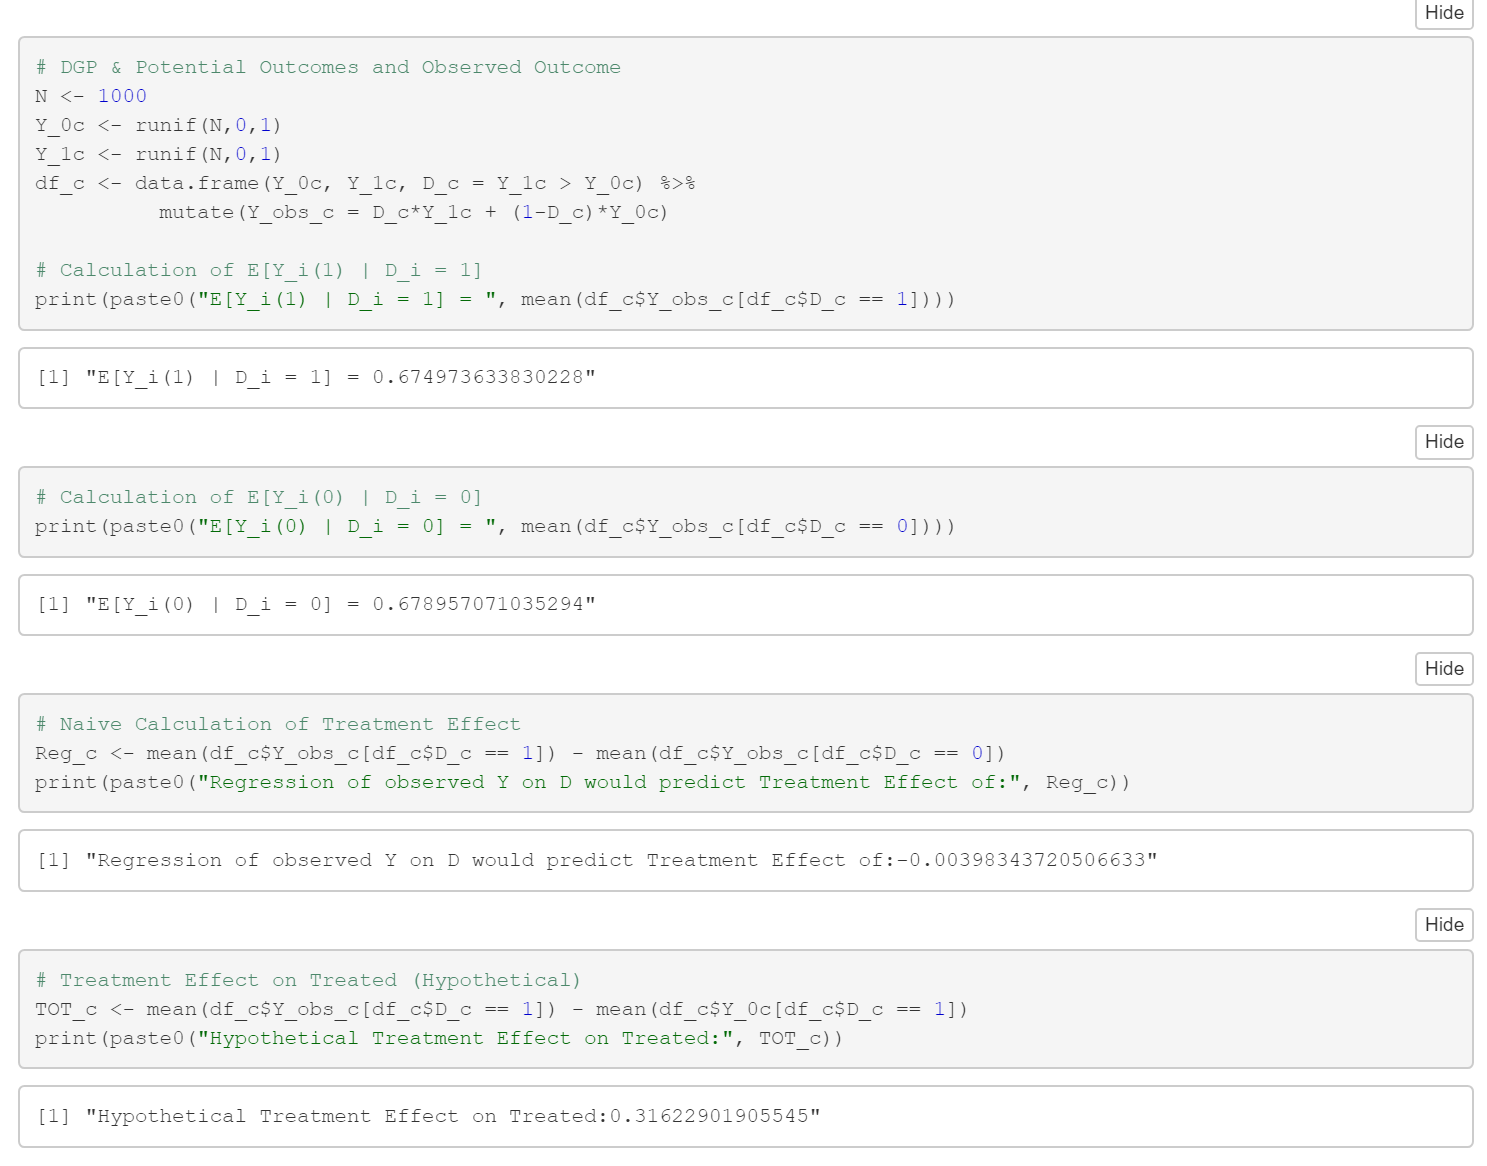
\includegraphics[width=15cm]{Q3c}
\end{figure}

Due to selection (lack of randomization of treatment), the treated group were of individuals who, if they could observe ex-ante their hypothetical outcomes in both states (treated and not treated) and compare, would clearly benefit from treatment. Hence, TOT will be positive.

If you now think about the group that selected into control / no treatment, it's the exact opposite. Their outcome is better off without treatment. If they were forced into treatment (instead of the others), their TOT would be negative.

Hence, expectation of observed outcomes at each level of D is higher than expectation of potential outcomes had there been randomization or equivalently had there been a way to observe everyone's potential outcomes in both treatment and control states.

This regression of Y on D would estimate no effect (if not negative), even though the hypothetical TOT is clearly positive.

%%%%%%%%%%%%%%%%%
%     Part d    %
%%%%%%%%%%%%%%%%%
\vem
\problem{}{
    \begin{enumerate}[label=(\alph*)*]
    \setcounter{enumi}{3}
        \item Now let $Y_i(0$) and $Y_i(1)$ be independent with marginal normal distributions with $\mu= 0$ and $\sigma^2= 0.5$.  Analytically derive $\E{Y_i(1) \cond D_i= 1}$ and $\E{Y(0)_i \cond D_i= 0}$. Does a regression of $Y_i$ on $D_i$ estimate TOT?
    \end{enumerate} 
}

% Below facts might be useful:
% \begin{itemize}
%     \item[1] From ARE 210, we know independent X and Y with marginal normality implies (X,Y) are jointly Normal. Given $Y_i(0) ~ N[0,0.5]$ , $Y_i(1) ~ N[0,0.5]$, and $Y_i(0) \independent Y_i(1)$, we have $(Y_i(0), Y_i(1)) \sim N(\mu, \Sigma)$, where $\mu = 
%     \begin{bmatrix}
%         0 \\
%         0
%     \end{bmatrix}$
%     and $\Sigma = 
%     \begin{bmatrix}
%         0.5 & 0 \\
%         0 & 0,5
%     \end{bmatrix}$
%     \item[2] Joint normality of $(Y_i(0), Y_i(1))$ implies CEF has to be linear.
% \end{itemize}

\begin{align*}
\intertext{Because $Y_i(0)$ and $Y_i(1)$ are independent and symmetrically distributed, we know $\P[Y_i(0) < Y_i(1)]=0.5$. Suppressing the $i$ for a moment, let $Y_k \equiv Y_i(k)$, then the conditional CDF of $Y_1$ is}
F_{Y_1|Y_0 > Y_1}(y) &= \P[Y_1 < y | Y_0 < Y_1] \\
    &= \frac{\P[Y_0 < Y_1 < y]}{\P[Y_0 < Y_1]} \\
    &=\frac{1}{\sfrac{1}{2}} \int_{-\infty}^{y} \left[\int_{-\infty}^{y_1} f(y_0, y_1) \; dy_0 \right] \; dy_1 \\
    &= 2 \int_{-\infty}^{y} \left[\int_{-\infty}^{y_1} \phi(y_0)\phi(y_1) \; dy_0 \right] \; dy_1 \\
    &= 2 \int_{-\infty}^{y} \left[\int_{-\infty}^{y_1} \phi(y_0) \; dy_0 \right]\phi(y_1) \; dy_1 \\
    &= 2 \int_{-\infty}^{y} \Phi(y_1) \phi(y_1) \; dy_1 \\
\intertext{}
f_{Y_1|Y_0 > Y_1}(y) &= \frac{d}{dy}F_{Y_1|Y_0 > Y_1}(y) \\
    &=  2\frac{d}{dy}\int_{-\infty}^{y} \Phi(y_1) \phi(y_1) \; dy_1 \\ 
    &=  2\Phi(y) \phi(y) \\ 
\intertext{}
\E{Y_1 \cond D_i= 1} &= \E{Y_1 \cond Y_1>Y_0} \\
    &= \int_{-\infty}^{\infty} y \ f_{Y_1|Y_0 > Y_1}(y) \ dy \\
    &= \int_{-\infty}^{\infty} y \ 2\Phi(y) \phi(y) \ dy \\
    &= \frac{\sigma}{\sqrt{\pi}} \quad\text{by mathematica}\\
\intertext{}
\E{Y_0 \cond D_i= 0} &= \E{Y_0 \cond Y_0>Y_1}
\shortintertext{By symmetry of the independent and identical distributions, we know this is equal to the previous expectation}
    &= \frac{\sigma}{\sqrt{\pi}}\\
\intertext{So the ATE is 0.}
\intertext{By the same reasoning as in part (b), }
\overline{\tau}_{TOT} &= \E{Y_i(1)-Y_i(0) | D_i = 1} \\
                      &= \E{Y_i(1)-Y_i(0) | \tau_i > 0} \\
                      &= \E{Y_i(1)-Y_i(0) | Y_i(1)-Y_i(0) > 0} \\
                      &> 0
\intertext{So the regression of Y on D does not give us TOT.}
\end{align*}



%%%%%%%%%%%%%%%%%
%     Part e    %
%%%%%%%%%%%%%%%%%
\vem
\problem{}{
    \begin{enumerate}[label=(\alph*)]
    \setcounter{enumi}{4}
        \item Write Monte Carlo simulation code to confirm your0answer to part $(d)$ (or, if you skipped  part  $(d)$,  to  determine  the  answer  numerically).   What  happens  if  you generate an error $\varepsilon_i$ that’s normally distributed with $\mu= 0$ and $\sigma^2= 1$ and add it to both $Y_i(0)$ and $Y_i(1)$ to create a positive correlation between the two.  Does the regression estimate TOT, and if not, is it upwardly biased or downwardly biased?
    \end{enumerate} 
}

Preamble which includes clearing the environment and setting seed is omitted.

\begin{figure}[h!tp]
    \centering
    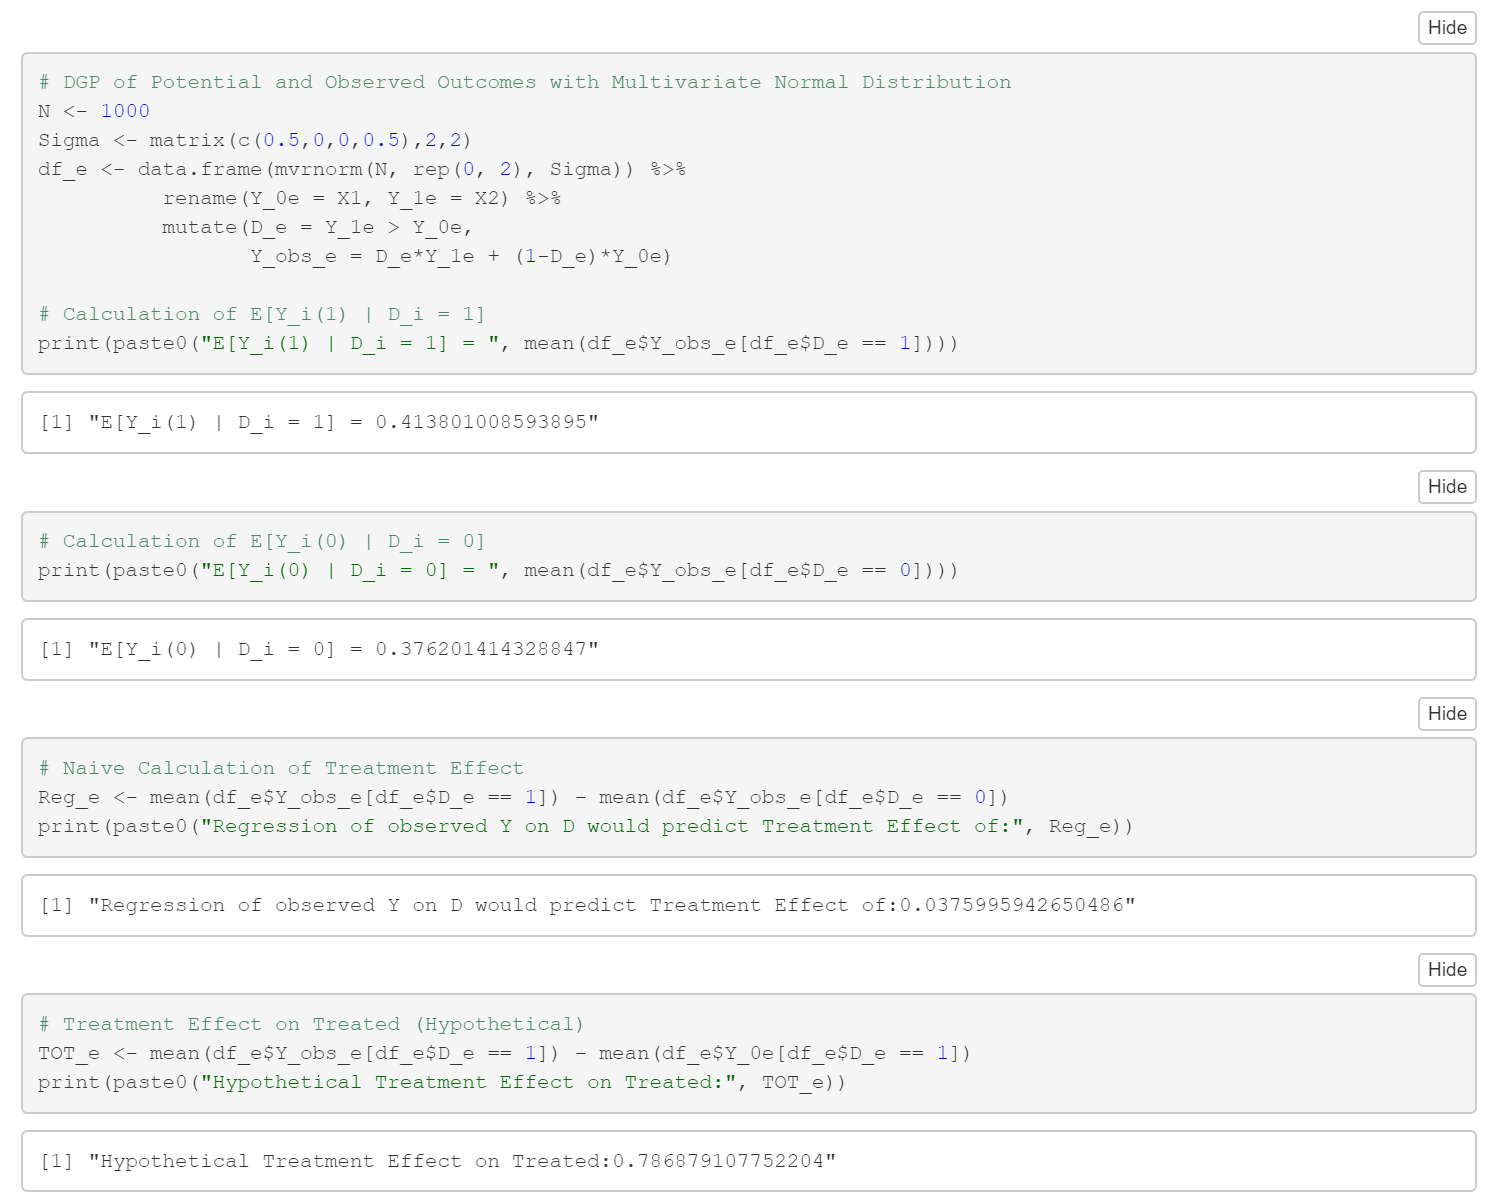
\includegraphics[width=15cm]{Q3e_p1}
\end{figure}

\begin{figure}[h!tp]
    \centering
    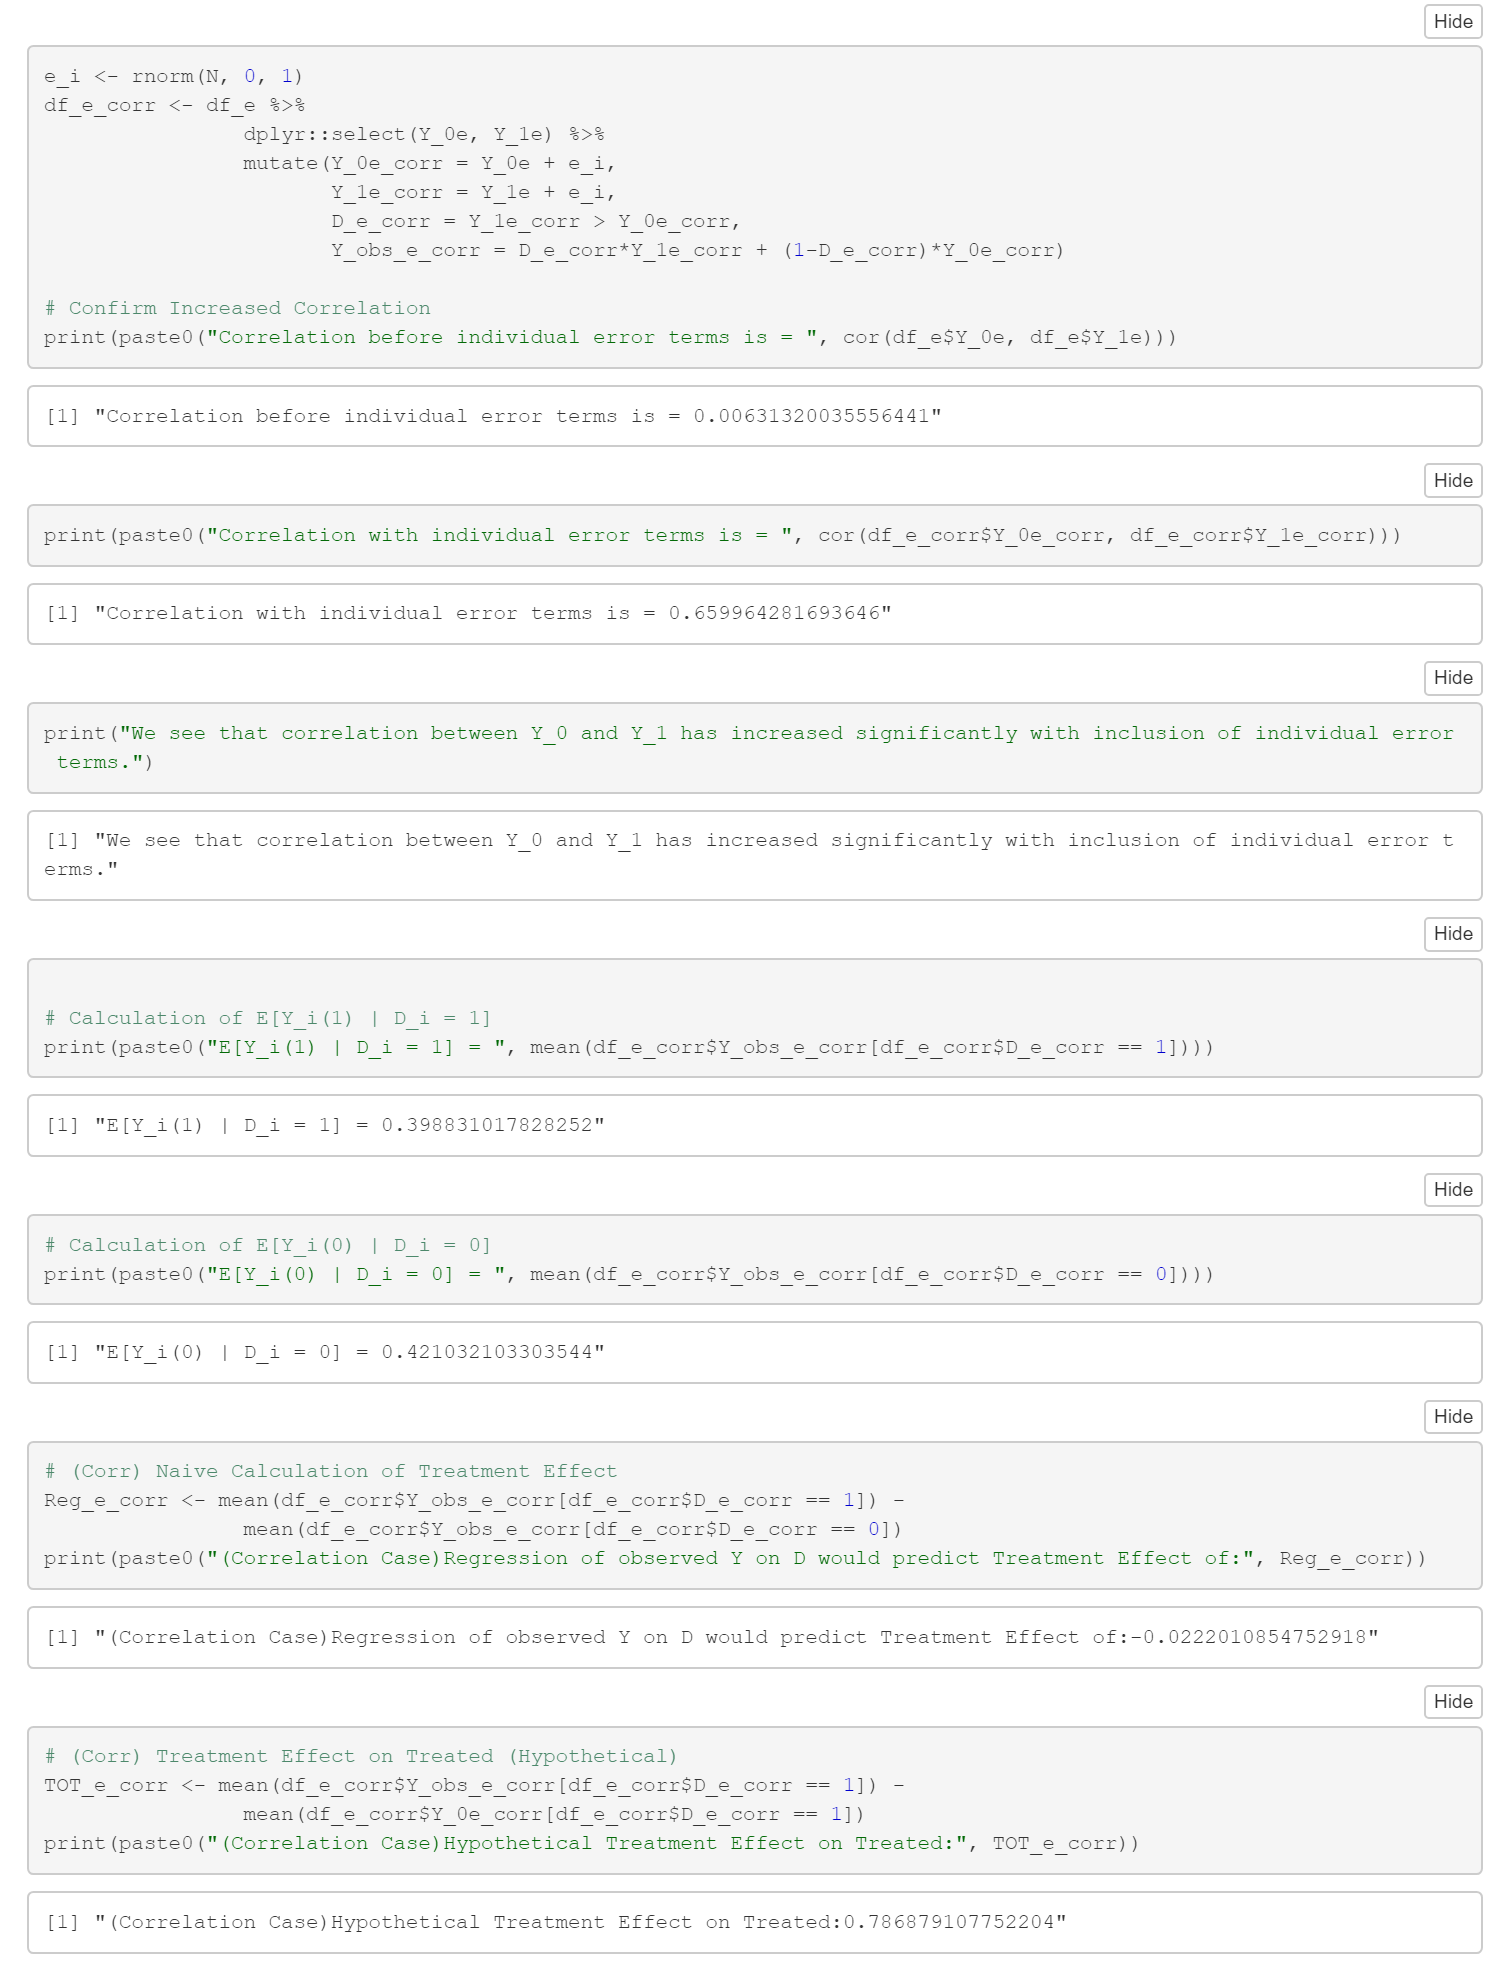
\includegraphics[width=15cm]{Q3e_p2}
\end{figure}
\FloatBarrier

Adding the error and making the two outcomes correlated only shifts both in the same direction. Again, this regression is downward-biased compared to actual TOT since both groups self-selected into the treatment and control. 

%%%%%%%%%%%%%%%%%
%     Part f    %
%%%%%%%%%%%%%%%%%
\vem
\problem{}{
    \begin{enumerate}[label=(\alph*)]
    \setcounter{enumi}{5}
        \item If  there  is  selection  bias  in  a  regression  of $Y_i$ on $D_i$,  is  it  positive  or  negative? How does the sign accord with your intuition about the general form of selection bias into, for example, getting a college degree (i.e.  a case in which $Y_i$ is later-life earnings and $D_i$ is whether the individual got a college degree).  What does this say about the most basic form of the Roy Model?
    \end{enumerate} 
}

Because of selection bias, the treated are precisely those who will experience a larger positive effect from the treatment than those who choose not to be treated. Not only that, but those in the control group selected to be in the control precisely because that is where \textit{they} would be better off. Thus, The selection bias in this regression of Y on D will be negative.


\end{document}

References
